% This text is proprietary.
% It's a part of presentation made by myself.
% It may not used commercial.
% The noncommercial use such as private and study is free
% Nov. 2006
% Author: Sascha Frank 
% University Freiburg 
% www.informatik.uni-freiburg.de/~frank/
%
% additional usepackage{beamerthemeshadow} is used
%  
%  \beamersetuncovermixins{\opaqueness<1>{25}}{\opaqueness<2->{15}}
%  with this the elements which were coming soon were only hinted
\documentclass{beamer}
\usepackage{beamerthemeshadow}
\usepackage[utf8]{inputenc}
\usepackage[T1]{fontenc}



\begin{document}
\title{Ardrand: The feasibility of the Arduino as a random number generator}  
\author{Benedikt Kristinsson \\Advisor: Ýmir Vigfússon}
\date{\today} 

\frame{\titlepage} 

%\frame{\frametitle{Table of contents}\tableofcontents} 


\section{Randomness} 
\frame{\frametitle{Randomness} 
  \begin{itemize}
  \item Hard on CPU \pause
  \item External sources needed \pause
    \begin{itemize}
    \item Hard drives \pause
    \item Radioactive decay \pause
    \item Atmospheric noise (RANDOM.ORG) \pause
    \item Intel RNG \pause
    \end{itemize}
  \item But why? \pause
  \end{itemize}
}



\subsection{Cryptography}

\subsection{Pseudo-Random Number Generator}
\frame{\frametitle{Pseudo-Random Number Generator}
  \begin{itemize}
  \item Auðkennislykilinn/RSA SecureID \pause

    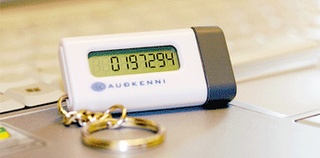
\includegraphics[scale=0.3]{img/lykill_1.png} \pause
    
  \item Deterministic \pause
  \item Only as secure as its seed \pause
  \item Unpredictable sequences \pause

  \end{itemize}
}

\frame{\frametitle{Cryptography}
  \begin{itemize}
    \item Bad seeding methods have resulted in breaking of cryptosystems \pause
      \begin{itemize}
      \item Netscape browser \pause
      \item Enigma \pause
      \end{itemize}
    \item Single-purpose devices \pause
  \end{itemize}
}

\section{How do we get entropy?} 

\frame{\frametitle{Possible ways}
\begin{itemize}
\item External hardware \pause
\item Obtain keys from outside \pause
\item Need \pause
  \begin{itemize}
  \item Available hardware \pause
  \item Cheap \pause
  \item Statistically sound \pause
  \item Fast \pause
  \end{itemize}
\end{itemize} 
}

\section{Today: Arduino}
\frame{\frametitle{Today: Arduino}
\centering
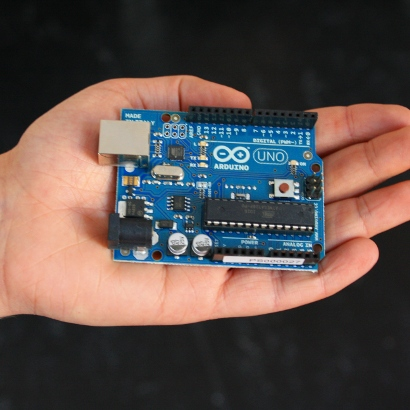
\includegraphics[scale=0.3]{img/arduino_uno_test.jpg}
}

\subsection{Arduino}
\frame{\frametitle{Arduino}
\begin{itemize}
\item Available \pause
\item Cheap (\$30) \pause
\item Analog noise from \texttt{analogRead} \pause
\item Does it work ? \pause
\item Is it fast enough? \pause
\item Has it been tried before? \pause

\end{itemize} 
\begin{quote}
If it is important for a sequence of [random] values generated to differ [...] initialize the random number generator with a fairly random input, such as analogRead() on an unconnected pin. 
\end{quote}
}


\subsection{Hypothesis}
\frame{\frametitle{Hypothesis}
  Hypothesis: Values returned from \texttt{analogRead} are random \pause

  \begin{itemize}
  \item Need stats! \pause
  \item Need an controlled environment (Iceland vs. Azerbaijan) \pause
  \end{itemize}

}
 
\section{Analysis}
\frame{\frametitle{Analysis}
  \begin{enumerate}
  \item Obtain sequences \pause
  \item Algorithms used \pause
  \item Statistical tests \pause
  \end{enumerate}

}

\section{Obtaining numbers}
\subsection{Obtained numbers}
% \frame{\frametitle{Obtained numbers}
% \begin{itemize}
%  \item Odd locations \pause
%   \begin{itemize}
%   \item Freezer \pause
%   \item Fridge  \pause
%   \item On top of heating element \pause
%   \item Bathtub \pause
%   \end{itemize}
% \item Normal locations\pause 
%   \begin{itemize}
%   \item Rooms in flat \pause
%   \item CS lab \pause
%   \item Garage\pause 
%   \end{itemize}
  
% \end{itemize}
% }

\frame{\frametitle{Odd locations}
  \centering
  \pause 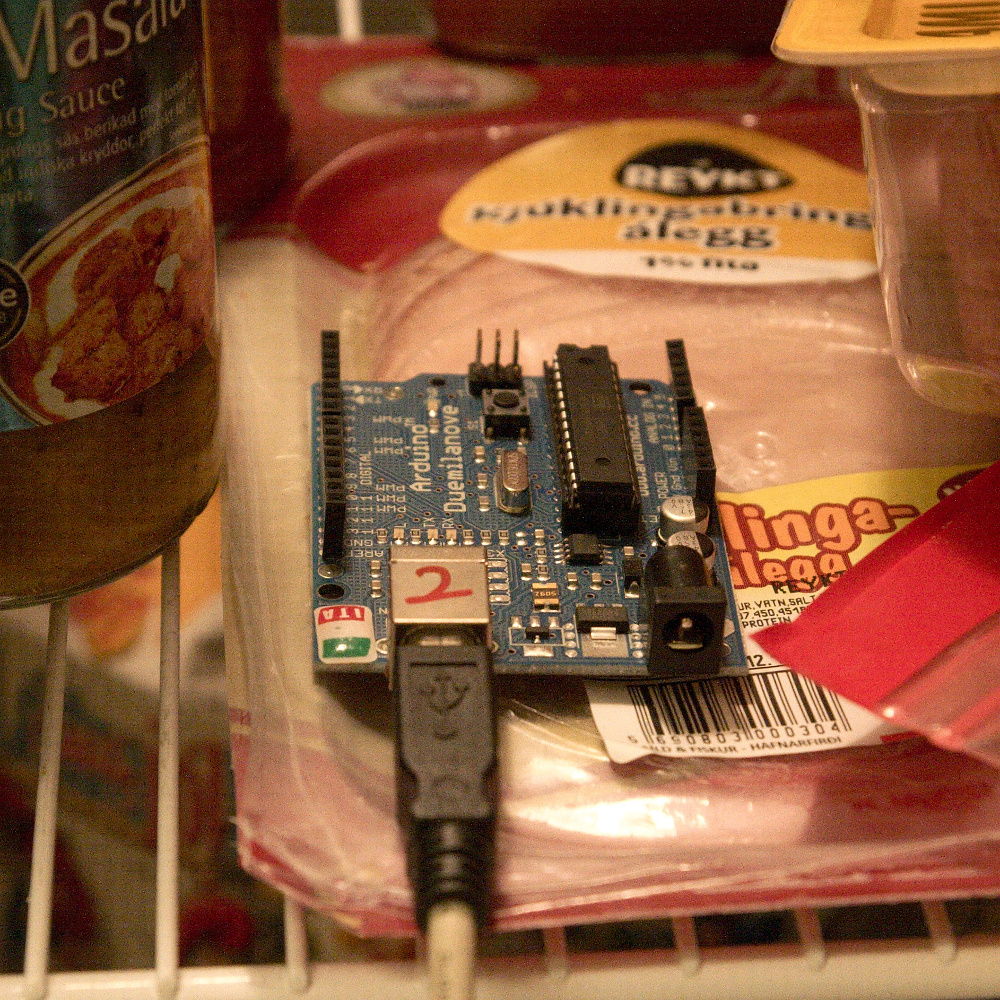
\includegraphics[scale=0.15]{img/ardfridge1.jpg} \pause
  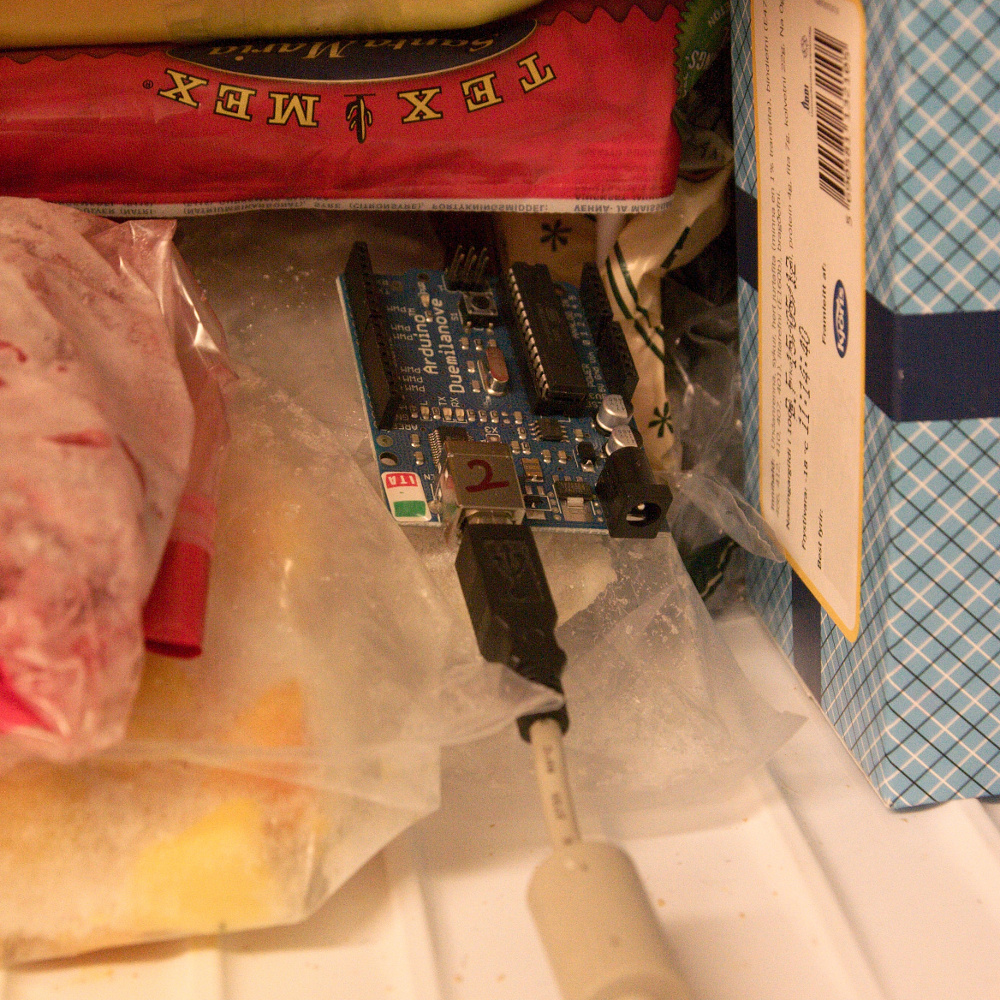
\includegraphics[scale=0.15]{img/ardfreezer1.jpg}
}

\frame{\frametitle{Odd locations}
  \centering
  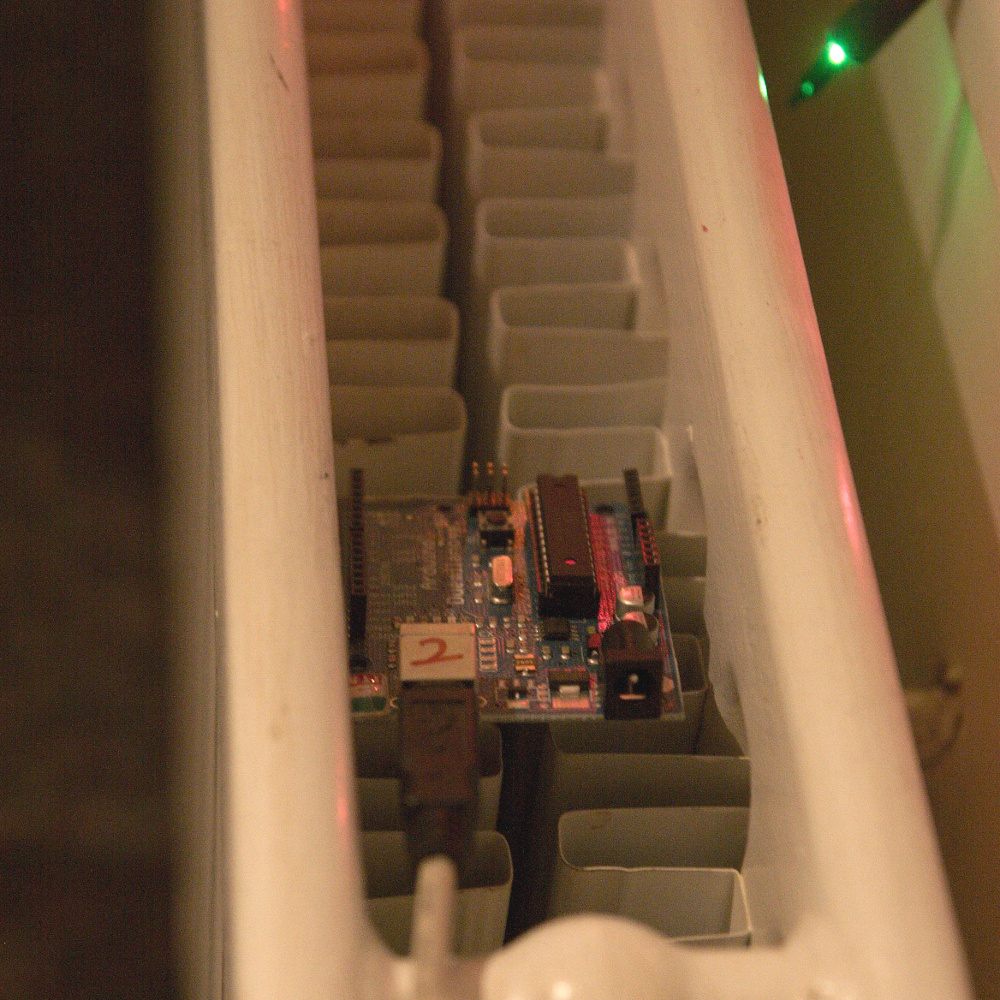
\includegraphics[scale=0.15]{img/ardonheating1.jpg} \pause
}

\subsection{Questions}
\frame{\frametitle{Questions}
  \begin{itemize}
  \item Q: Does the environment matter? \pause
  \item Q: How can we use the bits? \pause
  \item Q: How can we can for randomness? \pause
  \end{itemize}
}

\subsection{Does the environment matter?}
\frame{\frametitle{Does the environment matter?}
  Q: Does the environment matter? \pause
  
  \centering
  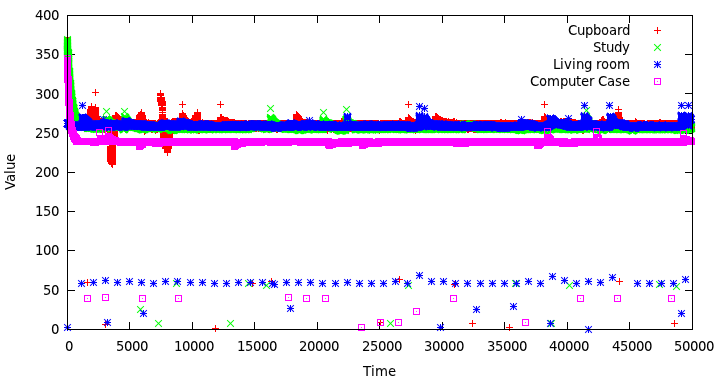
\includegraphics[scale=0.3]{img/environment.png} 

  Yes! 
}


\subsection{Temperature is important}
\frame{\frametitle{Temperature is important}

  \pause
  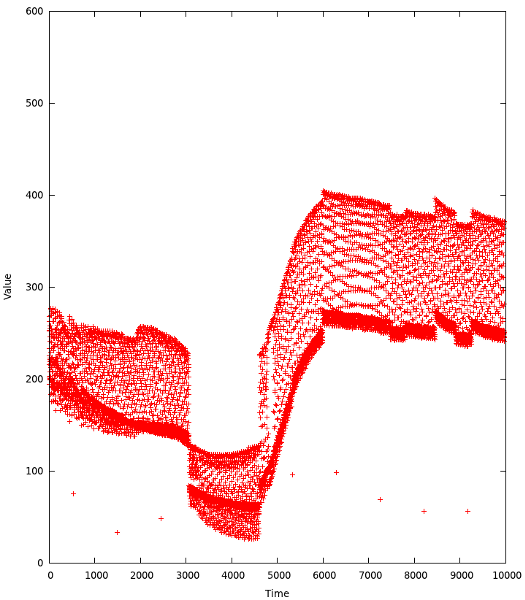
\includegraphics[scale=0.3]{img/freezer.png}
  \pause
  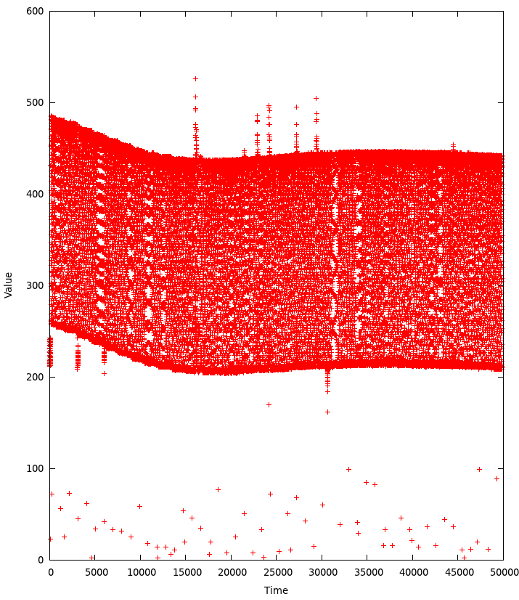
\includegraphics[scale=0.3]{img/heating.png}

  % \begin{figure}[h!]
  %   \centering  
  %   \subfloat[Sample from Ard3 taken on the desktop computer]{
  %     \label{fig:allpinsdesktop}
  %   }
  %   \subfloat[Sample from Ard3 taken on the D620]{
  %     \label{fig:allpinsd620}
  %   }

  %   \caption{Readings from Ard2 taken over all pins on both the desktop and D620 laptop}
  %   \label{fig:allpins}
        
  % \end{figure}

}



\section{Algoritms}
\subsection{The von Neumann box}
\frame{\frametitle{The von Neumann box}
  Used to remove bias from a generator \pause

  \begin{block}{Idea}
    Input two bits and discard them if they are the same. A 1,0-pair becomes a 1-bit and 0,1 pair becomes a 0-bit. 
  \end{block} \pause

  \begin{block}{Math}
    Let $p$ be the probability that the generator yields a 1-bit and $q$ that it yields a 0-bit. This relies on the fact that 01 and 10 are equiprobable since $p \cdot q = q \cdot p$.
  \end{block} \pause

  Applied in all our algorithms. 

}

\subsection{Meanrand}
\frame{\frametitle{Meanrand}

\begin{block}{Idea}
  Keep track of the mean of the values read, generate a 0 if below and a 1 otherwise. 
\end{block} 

\begin{itemize}
\item Observed bitrate: 25-85 bps \pause
\item Slow and not very random \pause
\end{itemize}
}

\subsection{Updownrand}
\frame{\frametitle{Updownrand}

  \begin{block}{Idea}
    Read one value. Generate a 1 bit if the next value is higher and a 0 bit otherwise. 
  \end{block} \pause
  
  \begin{itemize}
  \item Observed bitrate: 4 bps \pause
  \item Rejected: too slow \pause
  \item Not very random 
  \end{itemize}
}

\subsection{Mixmeanupdownrand}
\frame{\frametitle{Mixmeanupdownrand}
  \begin{block}{Idea}
    See what happens if we mix \texttt{Mean-RAND} and \texttt{Updown-RAND}. Generate one bit from either and XOR them together. 
  \end{block} \pause

  \begin{itemize}
  \item Observed bitrate: 2 bps \pause
  \item Rejected: too slow \pause
  \item Not very random either
  \end{itemize}

}

\subsection{Leastsignrand}
\frame{\frametitle{Leastsignrand}
  \begin{block}{Idea}
    Return the least significant (rightmost) bit for each value from \texttt{analogRead}
  \end{block} \pause

  \begin{block}{Math}
    Let $b = b_9, \ldots, b_1, b_0$ be a 10-bit integer generated by \texttt{analogRead}. Return $b_0$.
  \end{block} \pause
  
  \begin{itemize}
  \item Observed bitrate: 290 bps \pause
  \item Fastest \pause
  \item Passes most tests in some settings
  \end{itemize}

}

\subsection{Twoleastsignrand}
\frame{\frametitle{Twoleastsignrand}
  \begin{block}{Idea}
    Return the XOR of the two least significant (rightmost) bits for each value from \texttt{analogRead}
  \end{block} \pause

  \begin{block}{Math}
    Let $b = b_9, \ldots, b_1, b_0$ be a 10-bit integer generated by \texttt{analogRead}. Return $b_0 \oplus b_1$.
  \end{block} \pause
  

  \begin{itemize}
  \item Observed bitrate: $\approx 170$ bps \pause
  \item Second fastest, but not fast enough \pause
  \item Passes all tests in some settings
  \end{itemize}

}


\section{The statistical tests}
\frame{\frametitle{Statistical testing}
  \begin{itemize}
  \item Impossible to prove that a generator is random [AJM, PO, SA, 1996] \pause
  \item Not rejected rather than accepted as random \pause
  \item FIPS boundaries \pause
  \item 20,000 bits
  \end{itemize}
}

\subsection{Monobit test}
\frame{\frametitle{Monobit}
  \begin{block}{Idea}
    A random sequences should contain roughly the same number of 1's and 0's. This gives a statistic on this ratio. 
  \end{block} \pause

  \begin{block}{Math}
    Let $n_0$ denote the number of 0's and $n_1$ the number of 1's. We then find
    \[
    X_1 = \frac{(n_0 - n_1)^2}{2}
    \]
  \end{block}
}

\frame{\frametitle{Results}
  \begin{block}{Results}
    \begin{description}
    \item[Passed]
      \begin{itemize}
      \item \texttt{Mean-RAND} on all our computers \pause
      \item \texttt{Leastsign-RAND} on all our computers \pause
      \item \texttt{Twoleastsign-RAND} on all our computers \pause
      \end{itemize}
    \item[Rejected]
      \begin{itemize}
      \item \texttt{Updown} \pause
      \item \texttt{MixMeanUpdown}  (inconsistently) \pause
      \end{itemize}
    \end{description}
   
  \end{block}
}

\subsection{Poker test}
\frame{\frametitle{Poker test}
  \begin{block}{Idea}
    Based on the idea of five-card hands in poker. In a random sequence we would expect each hand to show up about the same amount of time. 
  \end{block} \pause

  \begin{block}{Math}
    Let $m$ be the size of the poker hand and $k = \lfloor \frac n m \rfloor$, where $n$ is the length of the sequence. Find

\[
X_3 = \frac{2^m}{k} \left( \sum_{i=1}^{2^m} n_i^2 \right) - k
\]
\end{block}
}


\frame{\frametitle{Results}
  \begin{block}{Results}
    \begin{description}
    \item[Passed]
      \begin{itemize}
        \item \texttt{Leastsign-RAND} on our laptops \pause
        \item \texttt{Twoleastsign-RAND} on our laptops \pause
      \end{itemize}
    \item[Rejected]
      \begin{itemize}

      \item \texttt{Updown-RAND} \pause
      \item \texttt{Mean-RAND} \pause
      \item \texttt{MixMeanUpdown-RAND} \pause
      \item All algoritms on desktop computer

      \end{itemize}
    \end{description}
   
  \end{block}
}


\subsection{Runs test}
\frame{\frametitle{Runs}
  
  \begin{block}{Runs examples}
    \texttt{100011} \pause
    \begin{itemize}
    \item Has one run (gap) of length 3 (three zeroes) \pause
    \item One run (block) of length 2 \pause
    \item One run of length 1 \pause
    \end{itemize}
  \end{block} \pause

  \begin{block}{Idea}
    Find the number of runs of each length. The longer the run, the unlikelier it is. The FIPS publication has a nice table listing how many sequences of each length should appear. 
  \end{block} \pause
}

\frame{
  \begin{block}{Math}
    Let $G_i$ and $B_i$ be the number of gaps and blocks of length i and $e_i$ denote the expected number of blocks of length $i$. Find
    \[
    X_4 = \sum_{i=1}^k \frac{(B_i - e_i)^2}{e_i} + \sum_{i=1}^k \frac{(G_i - e_i)^2}{e_i}
    \]
  \end{block}
}

\frame{\frametitle{Results}
  \begin{block}{Results}
    \begin{description}
    \item[Passed]
      \begin{itemize}
        \item \texttt{Leastsign-RAND} sometimes on laptops
        \item \texttt{Twoleastsign-RAND} always on one laptop
        \item \texttt{Twoleastsign-RAND} sometimes on another laptop
      \end{itemize}
    \item[Rejected]
      \begin{itemize}

      \item \texttt{Updown-RAND}
      \item \texttt{Mean-RAND}
      \item \texttt{MixMeanUpdown-RAND}
      \item All algoritms on desktop computer

      \end{itemize}
    \end{description}
   
  \end{block}
}


\section{Results}
\frame{\frametitle{Results}
  \begin{tabular}{| l | l | l | l | l | l |}
    \hline
    Algorithm & Monobit & Poker & Runs & Long runs & Bandwidth\\
    \hline
    \hline
    \texttt{Leastsign} & \textcolor{green}{\textbf{\tiny ACC}}
    & \textcolor{green}{\textbf{\tiny ACC}}
    & \textcolor{red}{(\textbf{\tiny REJ})}
    & \textcolor{green}{\textbf{\tiny ACC}}
    & 290.55 bps \pause\\
    
    \texttt{Twoleastsign} & \textcolor{green}{\textbf{\tiny ACC}}
    & \textcolor{green}{\textbf{\tiny ACC}}
    & \textcolor{green}{\textbf{\tiny ACC}}
    & \textcolor{green}{\textbf{\tiny ACC}}
    & 172.0 bps \pause\\
    
    \texttt{Mean} & \textcolor{green}{\textbf{\tiny ACC}}
    & \textcolor{red}{\textbf{\tiny REJ}}
    & \textcolor{red}{\textbf{\tiny REJ}}
    & \textcolor{green}{\textbf{\tiny REJ}}
    & 25.32 bps \pause\\

    \texttt{Updown-RAND} & \textcolor{red}{\textbf{\tiny REJ}}
    & \textcolor{red}{\textbf{\tiny REJ}}
    & \textcolor{red}{\textbf{\tiny REJ}}
    & \textcolor{green}{\textbf{\tiny REJ}}
    & 4 bps \pause\\

    \texttt{MixMeanUpdown} & \textcolor{green}{\textbf{\tiny ACC}}
    & \textcolor{red}{\textbf{\tiny REJ}}
    & \textcolor{red}{\textbf{\tiny REJ}}
    & \textcolor{green}{\textbf{\tiny REJ}}
    & 2 bps \pause\\

    \hline
  \end{tabular} \pause

  \begin{itemize}
  \item \texttt{Twoleastsign} passes NIST tests as well when it passes our tests
  \end{itemize}
}

\subsection{What does this mean?}
\frame{\frametitle{What does this mean?}
  \begin{itemize}
  \item Arduino not a feasible target using our methods \pause
  \item We created a seed discovery program \pause
    \begin{itemize}
    \item Runs quickly (Mean: 1.6 seconds) \pause
    \item Always finds seed in our experiments (5000 sequences) \pause
    \item Almost always finds the seed \pause
    \end{itemize}
  \end{itemize}
}

\subsection{Future work}
\frame{\frametitle{Future work}
  \begin{itemize}
  \item Find out what factors cause it to pass tests \pause
    \begin{itemize}
    \item Stabilize if possible \pause
    \end{itemize}
  \item Implement more algorithms to look for entropy \pause
  \item Cheap and simple modifications of Arduino \pause
  \item Workshop \pause
  \end{itemize}
}

\frame{\frametitle{Thank you}
  \huge Thank you. Questions?
  }

\end{document}